\documentclass{article}
% \usepackage{../../../lib/latex/draculatheme}
\usepackage{import}
\documentclass{article}
\usepackage[paper=letterpaper,margin=2cm]{geometry}
\usepackage[utf8]{inputenc}
\usepackage[russian]{babel}
\usepackage[]{graphicx}
\usepackage[usenames]{color}
\usepackage{colortbl}
\usepackage{geometry}
\usepackage{xcolor}
\usepackage{hyperref}
\usepackage{../../lib/latex/listings-rust}
\usepackage{fontspec}
\setmonofont{JetBrains Mono}[Contextuals=Alternate,Ligatures = TeX,]
\usepackage{listings}
\usepackage{keycommand}
\usepackage{caption}

\setmainfont[
  Ligatures=TeX,
  Extension=.otf,
  BoldFont=cmunbx,
  ItalicFont=cmunti,
  BoldItalicFont=cmunbi,
]{cmunrm}
\setsansfont[
  Ligatures=TeX,
  Extension=.otf,
  BoldFont=cmunsx,
  ItalicFont=cmunsi,
]{cmunss}

\geometry{
  a4paper,
  top=25mm,
  right=30mm,
  bottom=25mm,
  left=30mm
}

\hypersetup{
  colorlinks=true,
  linkcolor=blue!50!red,
  urlcolor=blue!70!black
}

\captionsetup[lstlisting]{
  font={tt},
}

% based on Atom One Light
\lstset{
  language=Java,
  frame=single,
  basicstyle=\ttfamily\color[HTML]{383a42},
  columns=fullflexible,
  breaklines=true,
  numbers=left,
  frame=tab,
  postbreak=\mbox{\textcolor{red}{$\hookrightarrow$}\space},
  extendedchars=false,
  showspaces=false,
  showstringspaces=false,
  identifierstyle=\ttfamily\color[HTML]{4078f2},
  commentstyle=\color[HTML]{a0a1a7},
  stringstyle=\color[HTML]{50a14f},
  keywordstyle=\color[HTML]{a626a4},
  numberstyle=\ttfamily\color[HTML]{2c91af},
  rulecolor=\color[HTML]{383a42}
}

\lstdefinelanguage{XML}
{
  morestring=[b]",
  morestring=[s]{>}{<},
  morecomment=[s]{<?}{?>},
}

\newcommand{\code}[1]{
  \lstset{title=#1}
  \lstinputlisting{#1}
}
\newkeycommand{\itmo}[variant=aboba, labn=aboba, discipline=aboba, group=aboba, student=aboba,teacher=aboba, year=2022]{
  \begin{titlepage}
    \begin{center}
      \section*{
        Федеральное государственное автономное образовательное учреждение\\ высшего образования\\
        «Национальный исследовательский университет ИТМО»\\
        Факультет Программной Инженерии и Компьютерной Техники \\
       }
      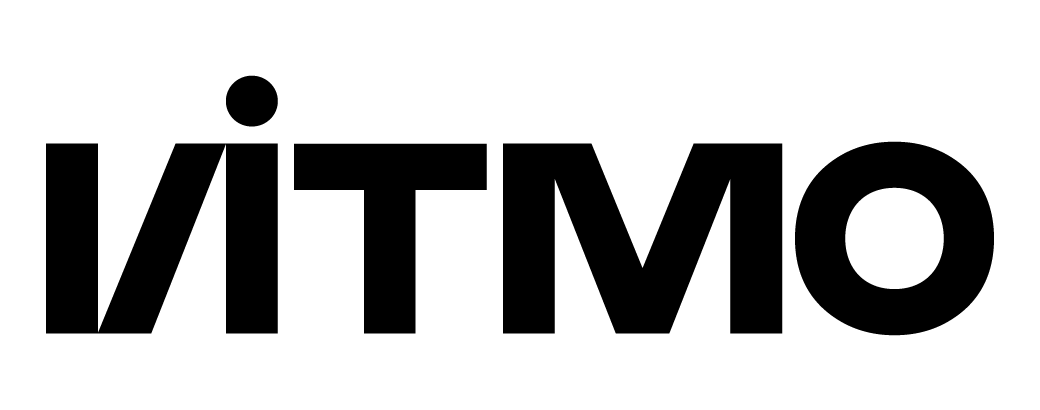
\includegraphics[scale=0.2]{../../lib/img/itmo.png}
    \end{center}

    \vspace{4cm}

    \begin{center}
      \large \textbf{Вариант \textnumero \commandkey{variant}}\\
      \textbf{Лабораторная работа \textnumero \commandkey{labn}}\\
      по дисциплине\\
      \textbf{\commandkey{discipline}}
    \end{center}

    \vspace*{\fill}

    \begin{flushright}
      Выполнил Студент группы \commandkey{group}\\
      \textbf{\commandkey{student}}\\
      Преподаватель: \\
      \textbf{\commandkey{teacher}}\\
    \end{flushright}

    \vspace{1cm}

    \begin{center}
      г. Санкт-Петербург\\
      \commandkey{year}г.
    \end{center}

    \thispagestyle{empty}
  \end{titlepage}
}



\begin{document}

\itmo[
  variant=74273,
  labn=5,
  discipline=Программирование,
  group=P3115,
  student=Владимир Мацюк,
  teacher=Кустарев Иван Павлович,
  year=2023,
  logo=../../../lib/img/itmo.png
]

\section*{Задание}

Реализовать консольное приложение, которое реализует управление коллекцией объектов в интерактивном режиме. В коллекции необходимо хранить объекты класса Product, описание которого приведено ниже.

\section*{Разработанная программа должна удовлетворять следующим требованиям:}
\begin{enumerate}
  \item Класс, коллекцией экземпляров которого управляет программа, должен реализовывать сортировку по умолчанию.
  \item Все требования к полям класса (указанные в виде комментариев) должны быть выполнены.
  \item Для хранения необходимо использовать коллекцию типа java.util.PriorityQueue
  \item При запуске приложения коллекция должна автоматически заполняться значениями из файла.
  \item Имя файла должно передаваться программе с помощью: аргумент командной строки.
  \item Данные должны храниться в файле в формате csv
  \item Чтение данных из файла необходимо реализовать с помощью класса java.util.Scanner
  \item Запись данных в файл необходимо реализовать с помощью класса java.io.FileWriter
  \item Все классы в программе должны быть задокументированы в формате javadoc.
  \item Программа должна корректно работать с неправильными данными (ошибки пользовательского ввода, отсутсвие прав доступа к файлу и т.п.).
\end{enumerate}

\section*{В интерактивном режиме программа должна поддерживать выполнение следующих команд:}
\begin{enumerate}
  \item help : вывести справку по доступным командам
  \item info : вывести в стандартный поток вывода информацию о коллекции (тип, дата инициализации, количество элементов и т.д.)
  \item show : вывести в стандартный поток вывода все элементы коллекции в строковом представлении
  \item add \{element\} : добавить новый элемент в коллекцию
  \item update id \{element\} : обновить значение элемента коллекции, id которого равен заданному
  \item remove\textunderscore by\textunderscore id id : удалить элемент из коллекции по его id
  \item clear : очистить коллекцию
  \item save : сохранить коллекцию в файл
  \item execute\textunderscore script file\textunderscore name : считать и исполнить скрипт из указанного файла. В скрипте содержатся команды в таком же виде, в котором их вводит пользователь в интерактивном режиме.
  \item exit : завершить программу (без сохранения в файл)
  \item remove\textunderscore first : удалить первый элемент из коллекции
  \item add\textunderscore if\textunderscore max \{element\} : добавить новый элемент в коллекцию, если его значение превышает значение наибольшего элемента этой коллекции
  \item remove\textunderscore greater \{element\} : удалить из коллекции все элементы, превышающие заданный
  \item min\textunderscore by\textunderscore manufacture\textunderscore cost : вывести любой объект из коллекции, значение поля manufactureCost которого является минимальным
  \item count\textunderscore less\textunderscore than\textunderscore owner owner : вывести количество элементов, значение поля owner которых меньше заданного
  \item filter\textunderscore contains\textunderscore name name : вывести элементы, значение поля name которых содержит заданную подстроку
\end{enumerate}

\section*{Формат ввода команд:}
\begin{enumerate}
  \item Все аргументы команды, являющиеся стандартными типами данных (примитивные типы, классы-оболочки, String, классы для хранения дат), должны вводиться в той же строке, что и имя команды.
  \item Все составные типы данных (объекты классов, хранящиеся в коллекции) должны вводиться по одному полю в строку.
  \item При вводе составных типов данных пользователю должно показываться приглашение к вводу, содержащее имя поля (например, "Введите дату рождения:")
  \item Если поле является enum'ом, то вводится имя одной из его констант (при этом список констант должен быть предварительно выведен).
  \item При некорректном пользовательском вводе (введена строка, не являющаяся именем константы в enum'е; введена строка вместо числа; введённое число не входит в указанные границы и т.п.) должно быть показано сообщение об ошибке и предложено повторить ввод поля.
  \item Для ввода значений null использовать пустую строку.
  \item Поля с комментарием "Значение этого поля должно генерироваться автоматически" не должны вводиться пользователем вручную при добавлении.
\end{enumerate}

\section*{Описание хранимых в коллекции классов:}
\begin{lstlisting}[language=java]
  
public class Product {
  private Long id; //Поле не может быть null, Значение поля должно быть больше 0, Значение этого поля должно быть уникальным, Значение этого поля должно генерироваться автоматически
  private String name; //Поле не может быть null, Строка не может быть пустой
  private Coordinates coordinates; //Поле не может быть null
  private java.time.ZonedDateTime creationDate; //Поле не может быть null, Значение этого поля должно генерироваться автоматически
  private double price; //Значение поля должно быть больше 0
  private float manufactureCost;
  private UnitOfMeasure unitOfMeasure; //Поле может быть null
  private Person owner; //Поле не может быть null
}
public class Coordinates {
  private float x;
  private Long y; //Поле не может быть null
}
public class Person {
  private String name; //Поле не может быть null, Строка не может быть пустой
  private java.time.LocalDateTime birthday; //Поле может быть null
  private Country nationality; //Поле не может быть null
}
public enum UnitOfMeasure {
  SQUARE_METERS,
  LITERS,
  GRAMS;
}
public enum Country {
  CHINA,
  SOUTH_KOREA,
  JAPAN;
}
\end{lstlisting}

\section*{Диаграмма классов}

\begin{center}
  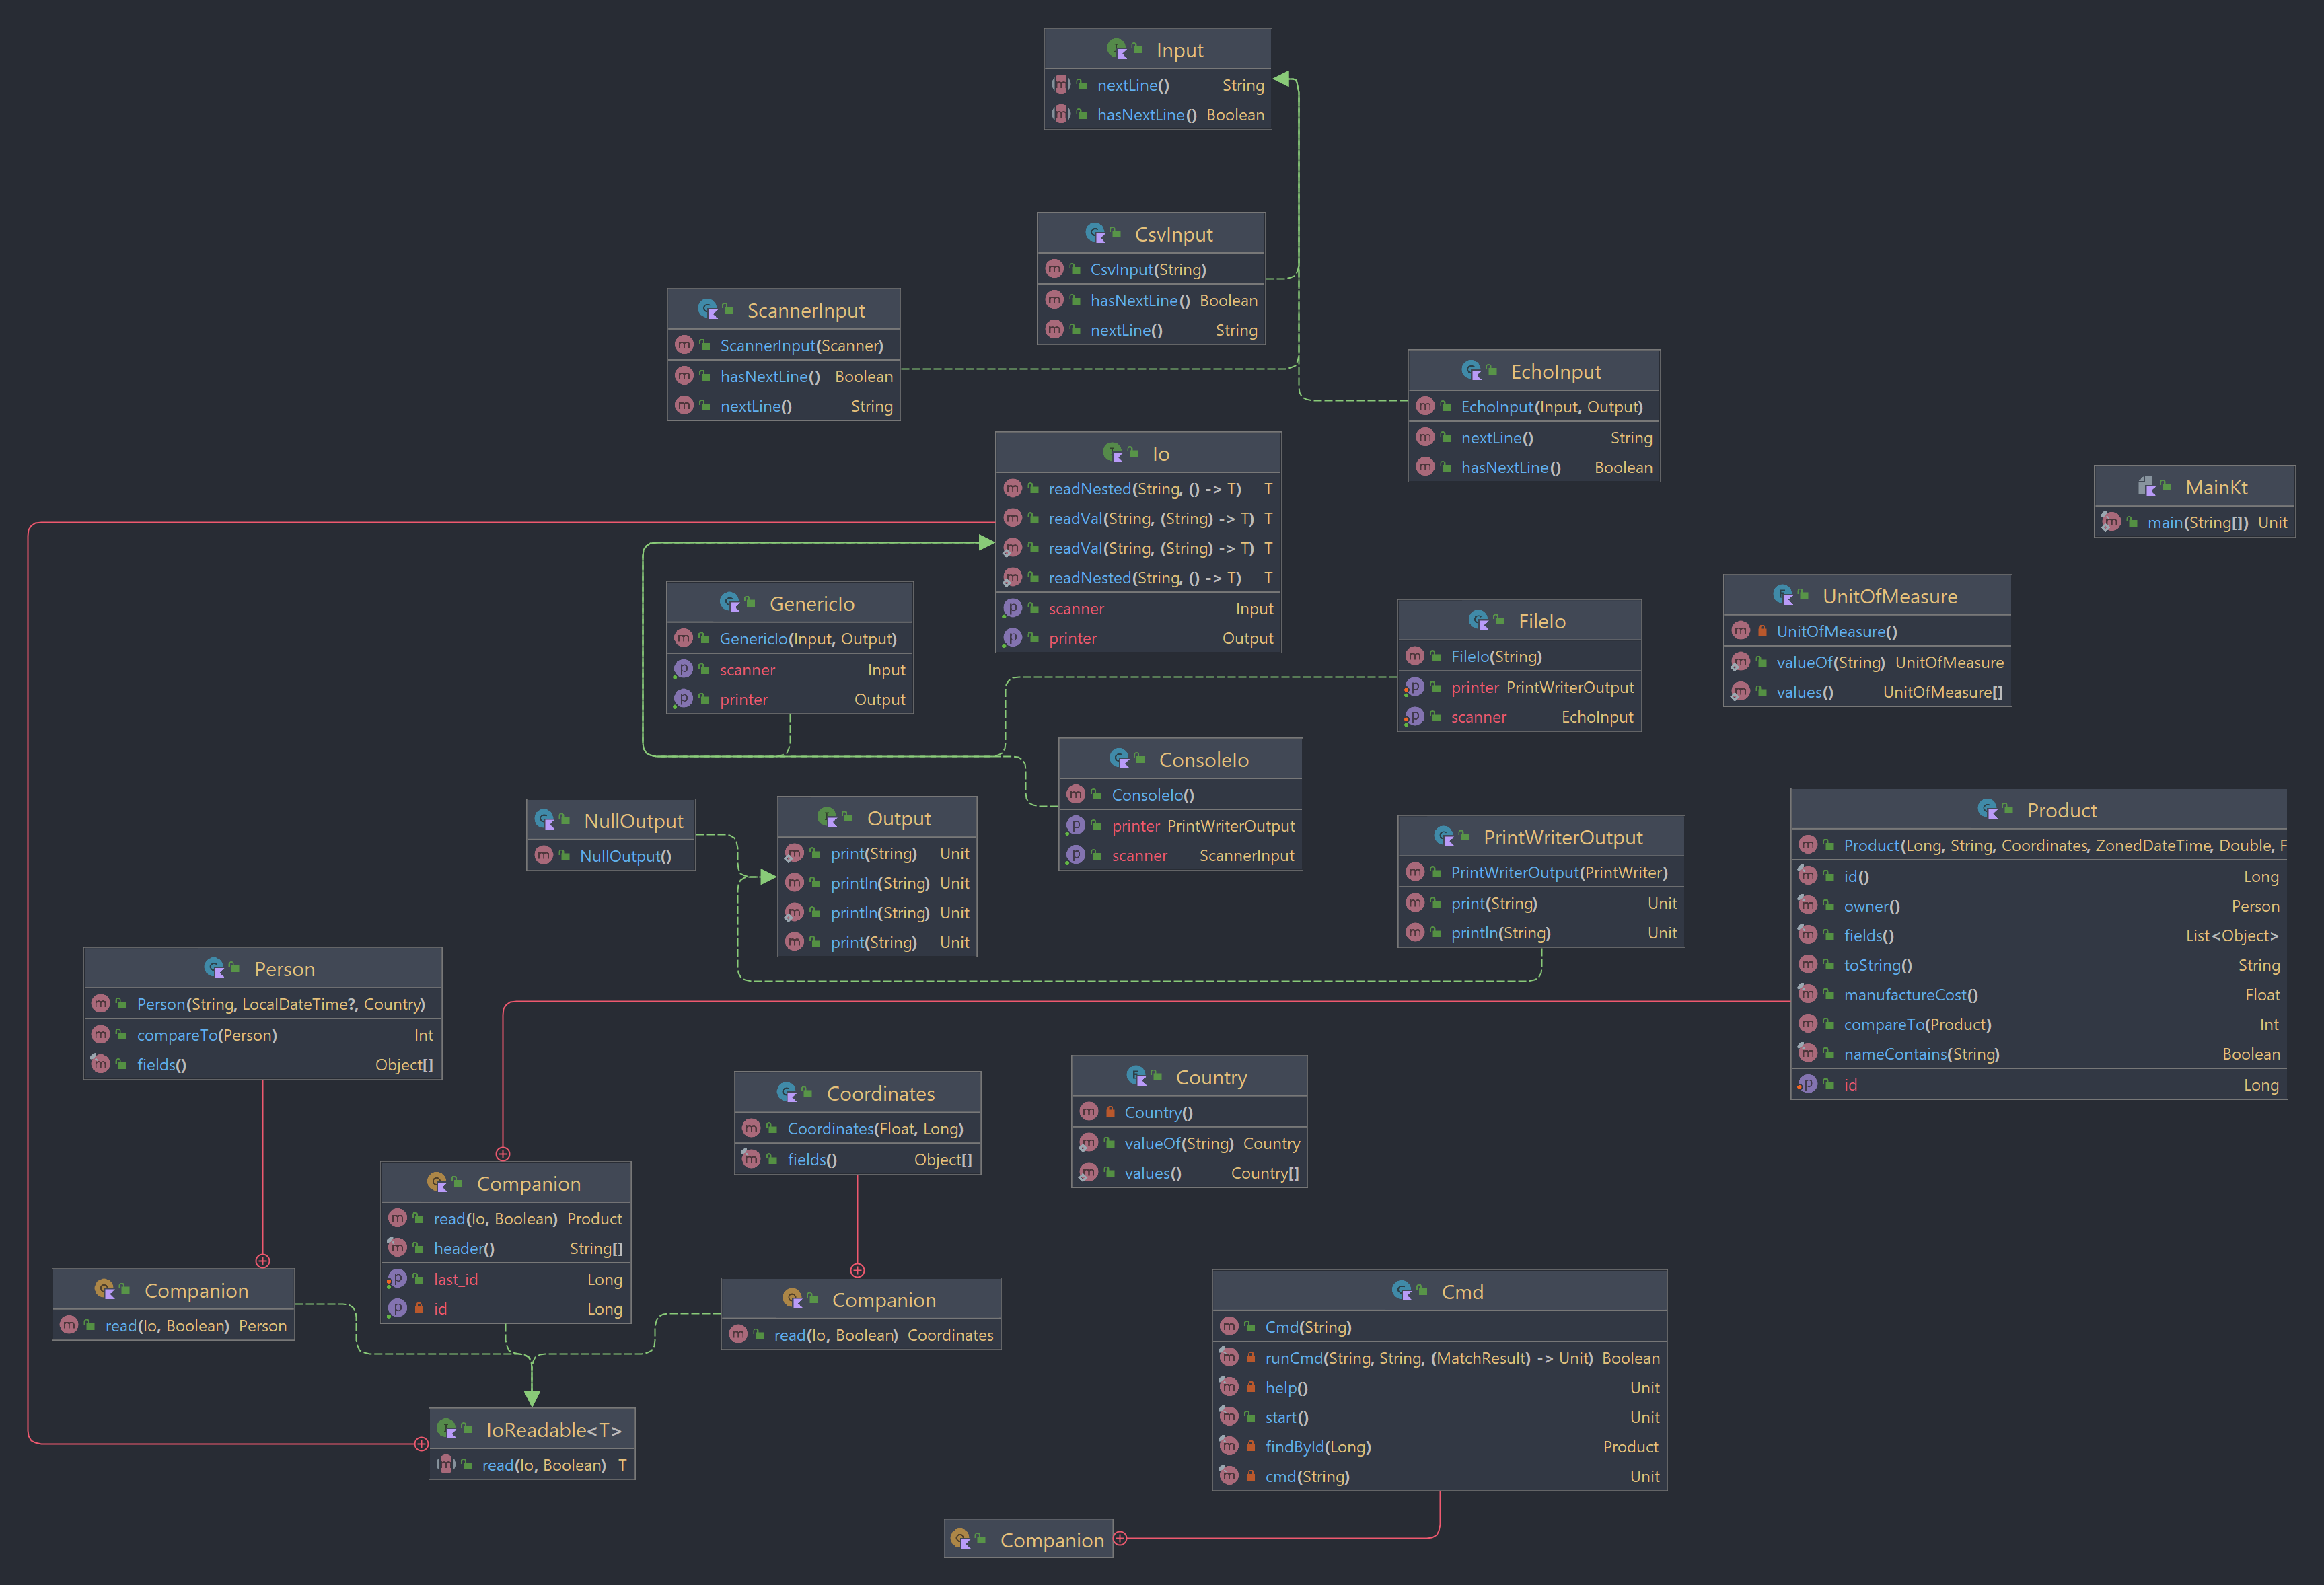
\includegraphics[scale=0.15]{diagram.png}
\end{center}

\section*{Исходный код}
\url{https://github.com/Wgmlgz/itmo2/tree/main/l5}

\section*{Вывод}
Во время выполнения работы я глубже ознакомился с ООП на языке java.
\end{document}
